\chapter{Projects}
\glsresetall

\section{Reinforcement Learning Research Paper}

At the start of my placement, my first project was to contribute to a research paper the company had
been working on. The subject of the paper revolved around \acro{ml}, \acrodesc{ml}.

As the company has a heavy focus on robotics, the paper focuses specifically on the application of
\acro{rl} on robotics. It is \acrodesc{rl}. As explained in \textcite{sutton2018reinforcement}, this
differs from other \acro{ml} approaches which focus on labelling unseen data based on previous
examples (Supervised Learning), or inferring structure and relations from unlabelled data
(Unsupervised Learning). In robotics, \acro{rl} is preferred over other \acro{ml} methods as it
allows for robots to learn and adapt complex behaviours from unstructured environments via the
\enquote{trial and error} method, without having to provide examples of the numerous complex
environments they could be deployed in.

Robotic environments commonly handle non-Euclidean data---\glsdesc*{noneuclidean}---for attributes
like orientations and stiffness measurement. However, common reinforcement learning methods work
under the premise of Euclidean data---\glsdesc*{euclidean}---being used. This mismatch of data types
lead to non-Euclidean data being approximated under most contemporary methods. The paper's
contribution demonstrates a method to mitigate against this, by exploiting a specific non-Euclidean
mathematical construct (Riemannian geometry) in a way where data of non-Euclidean nature is
preserved during reinforcement learning training. Adapting these methods to be \enquote{geometry
    aware} can be shown to increase accuracy during training, resulting in better policies (solutions)
when applying reinforcement learning.

\begin{figure}
    \centering
    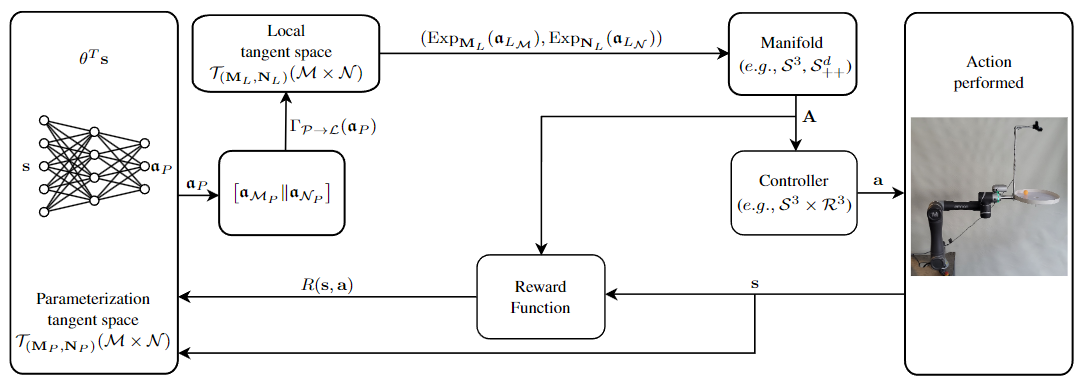
\includegraphics[width=\textwidth]{paper-pipeline}
    \caption{An illustration I created providing an overview of the proposed
        framework.\label{fig:paper-framework}}
\end{figure}

My specific role was to implement the theory of the paper in Python, run several experiments under
different environments comparing different approaches, generate accompanying visualizations, and
present my findings in the paper. As expected, this required extensive learning prior to me starting
my work. This came in the form of an online course provided by Coursera, which covered the
fundamentals of \acro{rl} from the works of \textcite{sutton2018reinforcement}. This was followed up
with an introduction to Deep RL---reinforcement learning via neural networks---by
\textcite{openai2018spinningup}.

Throughout my training, I gave presentations on these fundamental concepts and algorithms to other
colleagues, allowing me to receive valuable feedback in the areas I lacked clear explanations in and
helping me to evaluate gaps in my knowledge. My participation in the paper began when I had clearly
understood the fundamental premise of the paper along with some necessary background
knowledge.

This crash course in \acro{rl} was fairly enlightening, not only in academic knowledge, but also in
the effort it took to convey the knowledge in an accessible and understandable manner. Neither
presentation work nor essay writing were frequently exercised during my degree, and was therefore a
skill I had not exercised in a while. This would end up being a common theme during this project, as
the nature of a research paper is inherently to convey information in a manner which others can
understand.

Implementing the paper's proposed framework (Fig.~\ref{fig:paper-framework}) involved the
use of many technologies I had little experience with before. \gls*{pytorch}, \glsdesc*{pytorch},
was used in conjunction with \gls*{stablebaselines}, \glsdesc*{stablebaselines}, to reflect the
paper's proposal. I ran several experiments under simulation using the Gym Python library,
\glsdesc*{gympython}, to evaluate the paper's approach against several contemporary \acro{ml}
algorithms and other experimental approaches.

This was a moderately challenging task, with many issues arising that I had not anticipated.
Ensuring my implementation of the paper was mathematically valid was critical, and many weeks were
spent with my manager and other researchers on the paper to ensure this was the case. This involved
the usage of both black-box and white-box testing, with my code validated against Matlab code
written by the researchers as a proof-of-concept. As my confidence in knowledge built up, I
challenged colleagues on some aspects of the code I found confusing or questionable, and had
constructive conversations on the best way to implement certain aspects of the proposed approach.

Additionally, the speed of execution was fairly slow due to the heavy use of neural networks being
computationally restricted by hardware limitations. Deep \acro{rl} significantly benefits from
strong GPUs due to the vast amount of computation neural networks require, with faster GPUs being
able to better utilise parallel processing at a larger scale. To work around this limitation, I made
use of Google's Colaboratory service, specifically designed for neural network and ML research which
provides access to data centre GPU computation. This resulted in a considerable performance
increase; what once took a weekend to process was now able to be completed in a matter of hours.

\begin{figure}
    \centering
    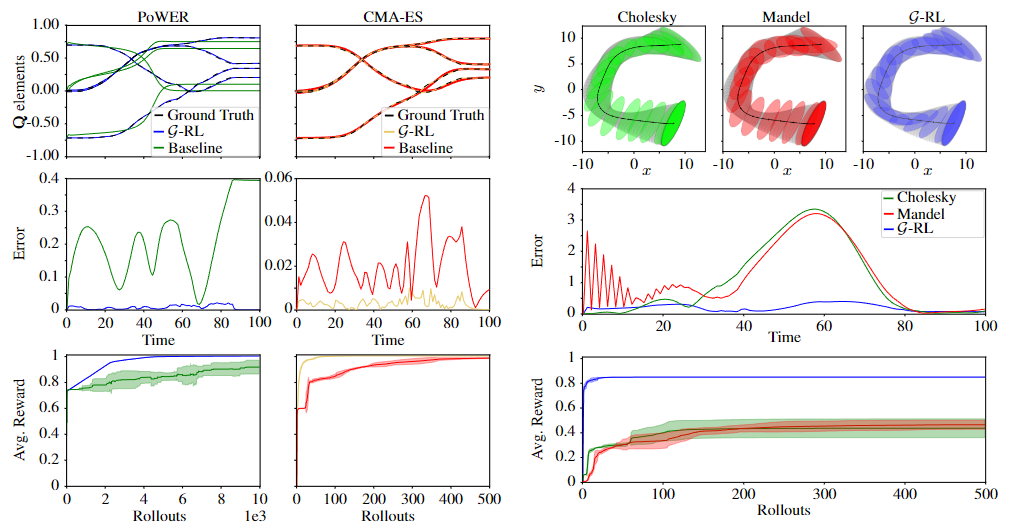
\includegraphics[width=\textwidth]{paper-results}
    \caption{A collection of graphs I created from experiment results.\label{fig:paper-figures}}
\end{figure}

The results of the experiments were presented using \gls*{matplotlib}, \glsdesc*{matplotlib}, with
accompanying graphics created in \gls*{inkscape}, \glsdesc*{inkscape}, as seen in
Fig.~\ref{fig:paper-figures}. These were inserted alongside the text of the paper, which was typeset
with \LaTeX.

An issue arose when collecting results as they had to be compiled from both Python and Matlab
codebases, across several machines (local and cloud-based). As Python and Matlab were saving results
in different data formats, I had to parse both into a common format which could then be read by
Pandas, \glsdesc*{pandaspython}. From this common format, I made use of Jupyter notebooks to
visualize and refine the resultant graphs to ensure they were clear to understand.

Although a straightforward problem to solve, this issue could have been completely avoided had some
more thought been put into how results would be collected, as everyone was focused on the
implementation of the experiments rather than the output format. A common generic format such as a
\texttt{.csv} would have made collecting and visualising the data significantly easier.

When receiving feedback on the graphs I had generated, I discovered that my manager was colour-blind
and struggled to distinguish between data on the graph. Taking accessibility into account was not
something I had planned for, which I swiftly rectified with colour-blind friendly colours.
Responsibility lay on me to explain and evaluate the results of the experiments in the paper. This
again fell back to my knowledge gained during this project and conveying it in a clear manner, while
also following editorial guidelines of the publisher. The content (along with the rest of the
paper) was reviewed by all authors of the paper before being sent for review.

This project allowed me to throw myself into the deep end of \acro{ml}, using libraries and
algorithms I had not used before. While very challenging, the problem-solving process was very
enjoyable and piqued my interest in a new area of computer science. It also gave an insight into
academia I had not experienced before, providing me with the opportunity to co-author a research
paper.

\section{Robot Manipulation Library}

As the company was moving towards in-house software solutions for robotic software control, I was
tasked to assist in developing a C++ manipulation library using the
\acro{ros}\footnote{Counter-intuitively, \acro{ros} is \emph{not} an operating system in the
    traditional sense.}, \acrodesc{ros}, and \gls*{tesseract}, \glsdesc*{tesseract}.

The purpose of the task was to assess whether \gls*{tesseract} could be a viable alternative
compared to another popular planning framework, MoveIt. In comparison to MoveIt which is heavily
dependent on \acro{ros}, \gls*{tesseract} was \enquote{designed to be light weight, limiting the
    number of dependencies, mainly only using standard [C++] libraries} \autocite{tesseractgithub}. If
possible to migrate to \gls*{tesseract}, the tight coupling and dependencies on \acro{ros} can be
significantly reduced. \gls*{tesseract} also holds other advantages over MoveIt, boasting the
ability to support dynamic reconfigurations at runtime.

The details of the task involved the creation of a library that could execute motion using
waypoints, and motion via real-time teleoperation (teleop), working in both cartesian space
(specifying a robot's end-effector in 3D coordinates) and joint space (specifying all of a robot's
joint orientations). The library also considered appropriately stopping motion when a joint limit is
reached, while being adaptable to any generic robot arm.

To become comfortable programming with \acro{ros}, I worked on understanding the C++ tooling I would
be using (including build tools such as CMake and \acro{ros}-specific tools like \texttt{catkin}) as
well as going through several tutorials focusing on communication with simulated robots via
different methods, such as request-response and unidirectional observation data flows. I also tested
the trajectory controller (middleware to issue commands to robots) that I would end up using with
the library. The trajectory controller exposes a \enquote{goal} endpoint that accepts a trajectory
of joint positions across time. Once a goal is forwarded to the robot, the controller returns
several "feedback" states that correspond to the current progress of the action execution,
completing the action with a "result" state that indicates success or error.

Work on combining Tesseract and ROS began once I felt confident building on top of ROS. One major
hurdle with Tesseract is the notable lack of up-to-date documentation in the Tesseract project, from
installation to implementation. To aid in understanding, I began to document these processes in
order to aid myself and others. I also created a diagram illustrating the high-level details the
project required, highlighting areas needed to be implemented and areas that could depend on
Tesseract or ROS code.

By documenting my actions, I began to better appreciate the more well-documented code I've seen -
something I had previously took for granted. Many hours of frustration and debugging could have been
mitigated had basic documentation been available. Following this, efforts have been made to actively
document all aspects of my work, including personal projects.

As Tesseract is only a framework for motion planning, a planning algorithm still needed to be
selected for usage. My colleagues and I evaluated several different algorithm implementations
(primary ones being TrajOpt, OMPL, and Descartes). For each, we outlined the benefits and drawbacks
of each approach along with an evaluation of practical performance. For instance, the Descartes
planner is restricted to planning in Cartesian space, unlike the other planners available. TrajOpt
was notable in its ability to not only produce reliable trajectories under complex constraints, but
also in its ability to have initial conditions be seeded by other planners, providing more robust
solutions. Usage of TrajOpt also allowed for both joint space and Cartesian planning, as specific
constraints could be supplied to the algorithm depending on the type of motion required. TrajOpt was
therefore selected as the default planning algorithm, although it should be noted that Tesseract
supported the ability to change planners at runtime if a certain task was more suited towards
another planner.

I was also responsible for the implementation of real-time teleop in the library. While the
implementation of joint space teleop was relatively simple (adjusting the position value of a single
joint in response to user input), it was quite difficult to perform realtime Cartesian teleop as
moving along a line/axis involves the movement of all joints in a non-intuitive manner. My approach
to this problem was to use inverse kinematics (usage of kinematic equations to calculate joint
positions in order to reach a given end-effector position) to formulate a trajectory along a given
axis. Additionally, after searching through the Tesseract library code, I was able to apply
Tesseract's post-processing abilities onto my trajectory, ensuring a collision free trajectory and
allowing joint velocity values to be generated along side the IK positions. These were tested
vigorously by myself as well as others in simulation software (Gazebo) as well as on a physical
robot arm.

\begin{figure}
    \centering
    \begin{subfigure}{.5\textwidth}
        \centering
        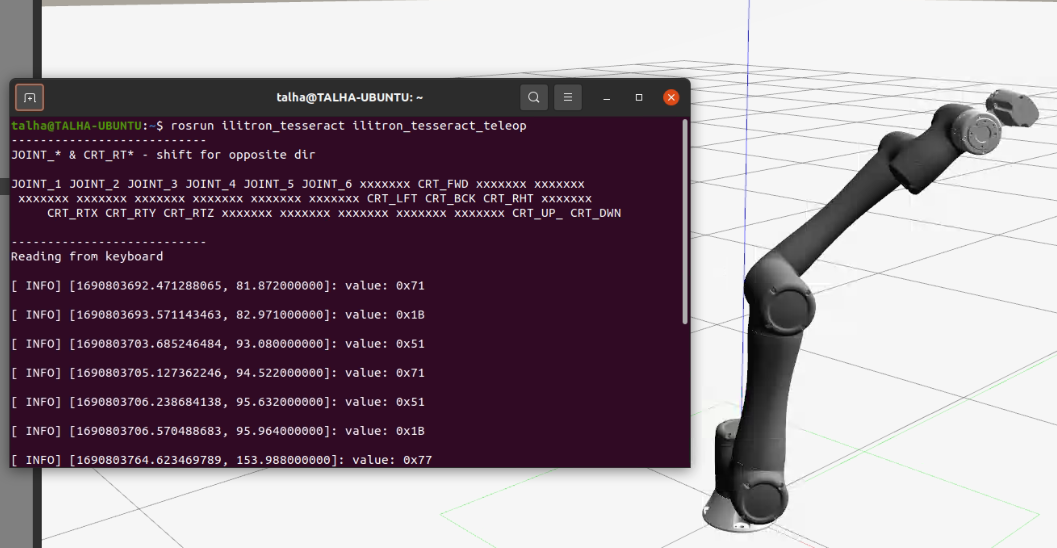
\includegraphics[width=.4\linewidth]{robot-tui}
        \caption{A subfigure}
        \label{fig:sub1}
    \end{subfigure}%
    \begin{subfigure}{.5\textwidth}
        \centering
        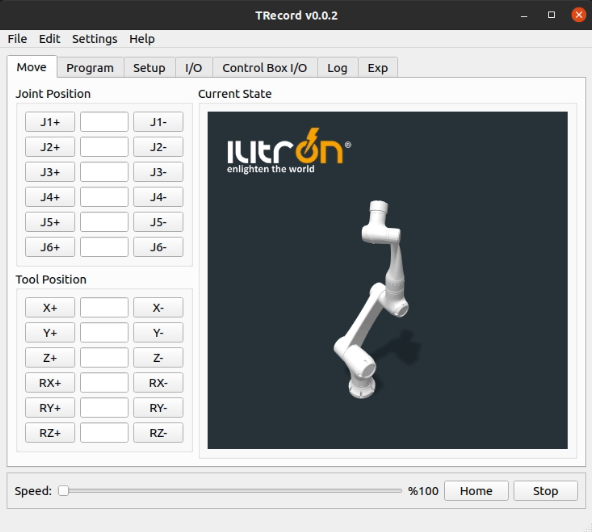
\includegraphics[width=.4\linewidth]{robot-gui}
        \caption{A subfigure}
        \label{fig:sub2}
    \end{subfigure}
    \caption{A figure with two subfigures}
    \label{fig:test}
\end{figure}

During this project I realized how imperative testing is in these safety-critical situations, as
numerous fail-safes - some of which I triggered - were put in place to prevent unexpected or
dangerous movement when running my teleop code on the physical arm. This ranged from software
measures to avoid self-collision and halt movement before irregular velocities or positions were
reached, as well as physical measures such as having more than one person observing the robot.
Coming from a background of no robotics or embedded software development, this was an aspect of
software I had never encountered before and taught me how different testing can be.

\section{Other projects}

\subsection{Task Management Web Application}

\subsection{EU HORIZON Proposal}

